\documentclass[12pt,a4paper]{article}
\usepackage[utf8]{inputenc}
\usepackage{amsmath}
\usepackage{amsfonts}
\usepackage{amssymb}
\usepackage{graphicx}
\usepackage{subcaption}
\usepackage{float}
\usepackage{multirow}
\usepackage{rotating}

\author{Team Gamma \\ {\small Ajda Frankovič, Martin Preradović, Niki Bizjak}}
\title{Face recognition}
\date{}
\begin{document}
    \maketitle

    In our third homework we were training a classifier to recognize 21 different faces.

    \section{Preparing training and testing data}

    \subsection{Obtaining images}

    This time we needed images of faces under different conditions. We took about 30 photos of each prined face (about 650 in total) and about 50 photos of each face in gazebo (about 1000 in total). \\

    One set of images of printed faces was taken from 1m, 1.5m and 2m of distance under different viewing angles (0, 30, 45 degrees) in the daylight. We also took some photos at 60 degrees viewing angle and distance of 1m. 
    The other set of images of printed faces was taken form 1m distance at different viewing angles and under two levels of lower light.
    For consistency, we tried to take images in a way that the face is in the center of the image. \\

    Photos in gazebo were also taken from different viewing angles and from different distances from the faces. \\

    In total, we obtained around 1700 images of faces. Below we present a subset of our data.

    % add 4 photos of Gargamel from gazebo here and to the folder "images"
    \begin{figure}[H]
        \centering
        \includegraphics[width=.20\linewidth]{images/gargamel_outside_30_2m.jpg}
        \includegraphics[width=.20\linewidth]{images/gargamel_outside_0_15m.jpg}
        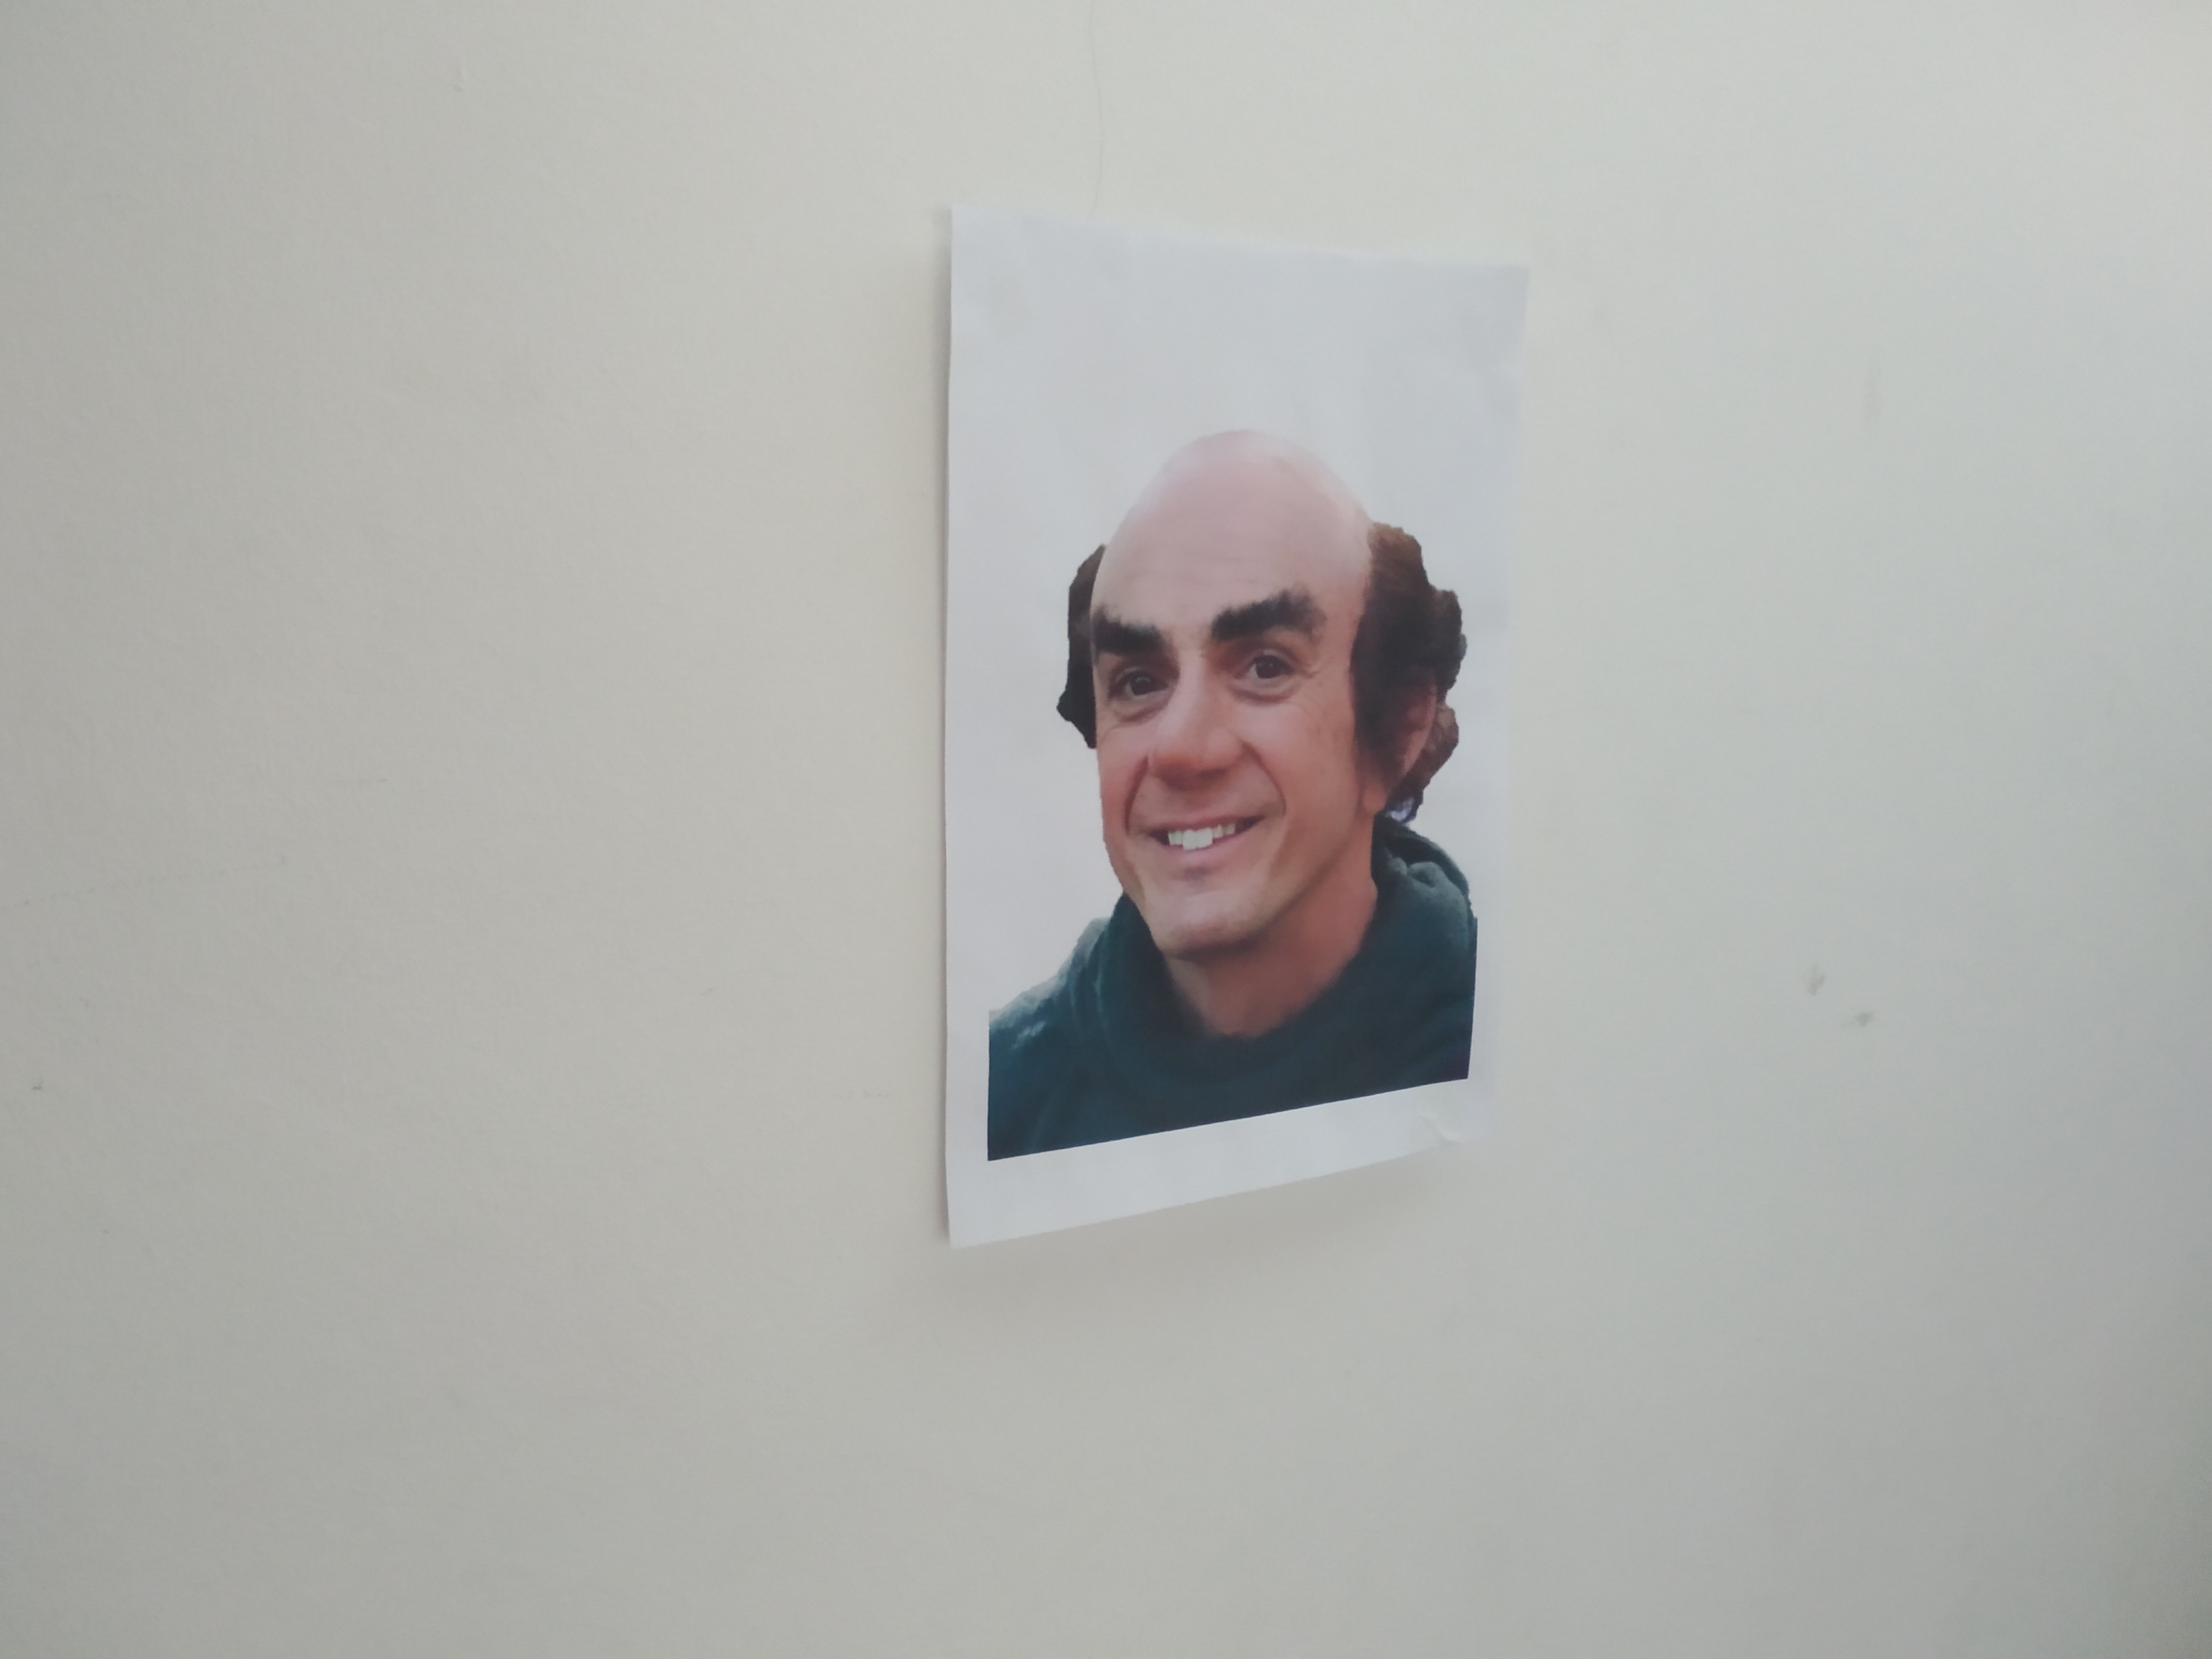
\includegraphics[width=.20\linewidth]{images/gargamel_inside_30_light.jpg}
        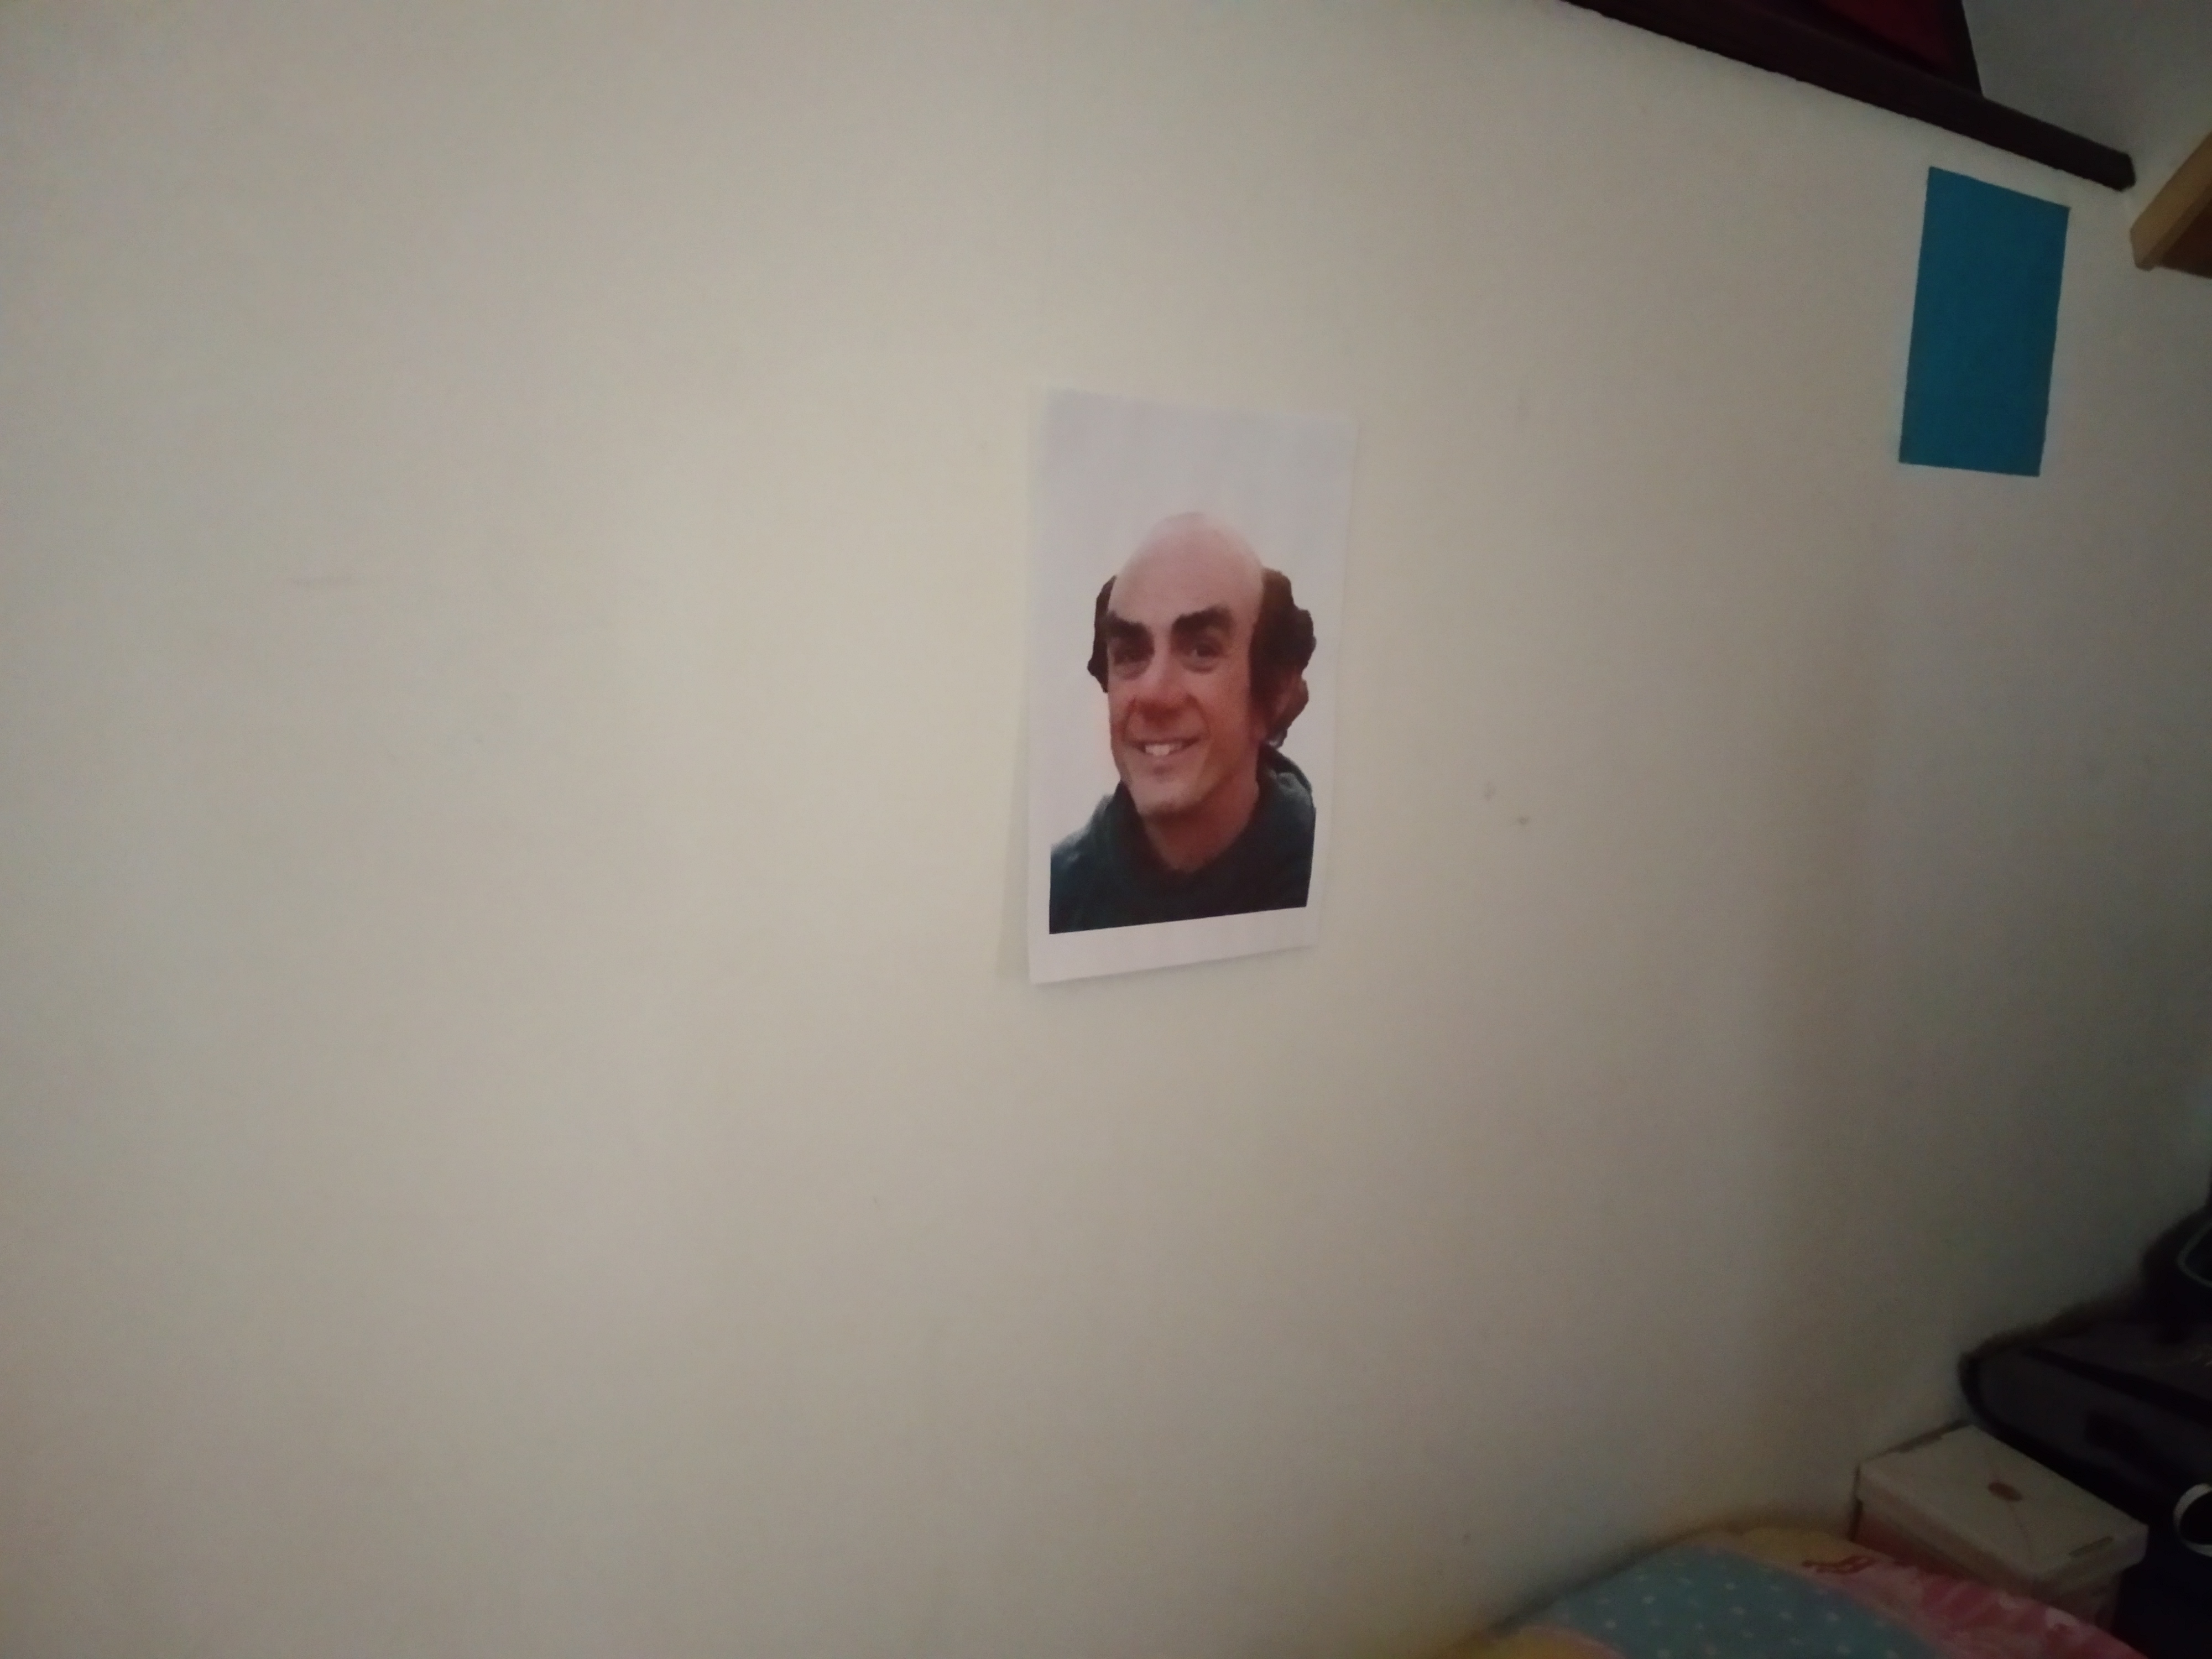
\includegraphics[width=.20\linewidth]{images/gargamel_inside_30_dark.jpg}
        \caption{Photos of faces}
    \end{figure}

    \subsection{Dividing images into training and testing set}

    We divided our images into the training and testing set in four different ways.

    \begin{enumerate} % a mogoce vemo, a je blo pol pol al kako drugo razmerje? To bi blo mogoč fajn vedet in dodat semle
		\item The set of images from gazebo was randomly split into training and testing set 
		\item The set of images of printed faces was randomly split into training and testing set
		\item Both sets of images were merged together into one, which was then randomly split in to training and testing set
		\item The set of images from gazebo was used as the training set and the set of images of printed faces was used as the testing set
    \end{enumerate}
    
    The fourth option performed awfully bad (about 42\% accuracy). For this reason we will only focus on the first three dataset partitions in the rest of the report. The bad performance isn't unexpected since images from gazebo contain less noise and blur then images of printed faces and are taken under consistent light conditions.

    \section{Training the classifier}

    \subsection{Preprocessing data}

    Data has to be preprocessed before it is given to the classifier, si it is consistent. On each image we detected a face and cropped out the part of image that contains the face. After that, image was translated (embedded) into 128-dimensional feature space such that similar faces translate to vectors that are close together in this feature space. These vectors were then given to the classifier with exception of knn classifier. For knn classifier, we performed additional step of normalizing the vectors, to ease the classification a little bit, since knn works worse on high-dimensional spaces.

    \subsection{Choosing a classifier}

    % what we chose/tried, why we thought this was a good idea. How it works.

    \section{Analysing the results}

    % accuracy of all tested classifiers, confusion matrix for the best classifier (or more best classifiers if the confusion matrix for the best shows that it is not actually the best), 
    % discussion on which hypotesis in "Choosing a calssifier" turned out to be true and which didn't. 
    % Why the accuracy isn't 100%? 
    % What will we use for our robot?

    In the table below, you can see the accuracy of each model on each of the partitions of our dataset into the training and testing set.
    \begin{enumerate}
		\item The set of images from gazebo was randomly split into training and testing set 
		\item The set of images of printed faces was randomly split into training and testing set
		\item Both sets of images were merged together into one, which was then randomly split in to training and testing set
    \end{enumerate}

    \begin{center}
        \begin{tabular}{|c|c|c|c|}
            \hline
			 & \multicolumn{3}{c|}{\textbf{Partition into training and testing set}} \\
			\hline 
			\textbf{Classifier} & \texttt{1.} & \texttt{2.} & \texttt{3.} \\
            \hline \hline
            
			\textbf{knn}, \small k = 3 & data goes here & and here & \textbf{this is bold} \\
			\textbf{knn}, \small k = 5 &  &  &  \\
			\textbf{knn}, \small k = 7 &  &  &  \\
			\hline \hline
			\textbf{decision tree}, \small gini &  &  &  \\
			\textbf{decision tree}, \small entropy &  &  &  \\
			\hline \hline
			\textbf{random forest}, \small gini &  &  &  \\
			\textbf{random forest}, \small entropy &  &  &  \\
			\hline \hline
			\textbf{naive bayes} &  &  &  \\
			\hline \hline
			\textbf{svm}, \small kernel=linear, c=0.025 &  &  &  \\
			\textbf{svm}, \small kernel=rbf, c=0.025 &  &  &  \\
			\textbf{svm}, \small kernel=linear, c=0.05 &  &  &  \\
			\textbf{svm}, \small kernel=linear, c=0.1 &  &  &  \\
			\textbf{svm}, \small kernel=linear, c=0.2 &  &  &  \\
			\hline
		\end{tabular} \\
    \end{center}
    
    % komentar na to, kaj opazimo v tabeli
     THIS IS JUST EXAMPLE TEXT: We can see that the Xth partiton has significantly higher scores with the cnn classifier than the other two. This is because the grass is green and because snakes exist. The overall best score is with Yth partition and XYZ classifier, which makes sense, since the images in the training set and those in the testing set share only a father but not also a mother and XYZ classifier works well on this kind of data. The wors performance can be seen with ABC classifier, which is a bit suprising. This probably happened because the chicken was not seasoned as usual but rather with some extra chili flakes. END OF EXAMPLE TEXT

     Since scores can only tell us this much, let's have a look at the confusion matrix for the best score, that is BLABLA classifier and BLABLA dataset partition. Gargamel is represented as \texttt{face01}.

    % If we have an image of the confusion matrix, insert it here, otherwise delete this part and use the table below
    \begin{figure}[H]
		\centering
		\includegraphics[width=1\linewidth]{images/Confusion_matrix.png}
		\caption{Confuson matrix for XYZ classifier used on ABC dataset partition}
    \end{figure}

    % delete if we have an image
     \begin{center}
        {\footnotesize
		\begin{tabular}{|c c c c c c c c c c c c c c c c c c c c c c c|}
			\hline
			\multicolumn{1}{|c}{} & \multicolumn{21}{c}{\multirow{2}{*}{\textbf{\large naive bayes on \texttt{HSV}}}} & \multicolumn{1}{c|}{}\\
			\multicolumn{1}{|c}{} & & & & & & & & & & & & & & & & & & & & & & \multicolumn{1}{c|}{}\\
			\hline
				& & \multicolumn{21}{|c|}{\textbf{predicted}} \\
				\multicolumn{2}{|c|}{}& \begin{sideways}face01\end{sideways} & \begin{sideways}face02\end{sideways} & \begin{sideways}face03\end{sideways} & \begin{sideways}face04 \end{sideways} & \begin{sideways}face05\end{sideways} & \begin{sideways}face06\end{sideways} & \begin{sideways}face07\end{sideways} & \begin{sideways}face08\end{sideways} & \begin{sideways}face09\end{sideways} & \begin{sideways}face10\end{sideways} & \begin{sideways}face11\end{sideways} & \begin{sideways}face12\end{sideways} & \begin{sideways}face13\end{sideways} & \begin{sideways}face14\end{sideways} & \begin{sideways}face15\end{sideways} & \begin{sideways}face16\end{sideways} & \begin{sideways}face17\end{sideways} & \begin{sideways}face18\end{sideways} & \begin{sideways}face19\end{sideways} & \begin{sideways}face20\end{sideways} & \begin{sideways}face21\end{sideways} \\ \hline
			\multirow{21}{*}{\begin{sideways}\textbf{actual}\end{sideways}}& \multicolumn{1}{c|}{01} & 0 & 0 & 0 & 0 & 0 & 0 & 0 & 0 & 0 & 0 & 0 & 0 & 0 & 0 & 0 & 0 & 0 & 0 & 0 & 0 & 0 \\
			&\multicolumn{1}{c|}{02} & 0 & 0 & 0 & 0 & 0 & 0 & 0 & 0 & 0 & 0 & 0 & 0 & 0 & 0 & 0 & 0 & 0 & 0 & 0 & 0 & 0 \\
			&\multicolumn{1}{c|}{03} & 0 & 0 & 0 & 0 & 0 & 0 & 0 & 0 & 0 & 0 & 0 & 0 & 0 & 0 & 0 & 0 & 0 & 0 & 0 & 0 & 0 \\
			&\multicolumn{1}{c|}{04} & 0 & 0 & 0 & 0 & 0 & 0 & 0 & 0 & 0 & 0 & 0 & 0 & 0 & 0 & 0 & 0 & 0 & 0 & 0 & 0 & 0 \\
			&\multicolumn{1}{c|}{05} & 0 & 0 & 0 & 0 & 0 & 0 & 0 & 0 & 0 & 0 & 0 & 0 & 0 & 0 & 0 & 0 & 0 & 0 & 0 & 0 & 0 \\
            &\multicolumn{1}{c|}{06} & 0 & 0 & 0 & 0 & 0 & 0 & 0 & 0 & 0 & 0 & 0 & 0 & 0 & 0 & 0 & 0 & 0 & 0 & 0 & 0 & 0 \\
            &\multicolumn{1}{c|}{07} & 0 & 0 & 0 & 0 & 0 & 0 & 0 & 0 & 0 & 0 & 0 & 0 & 0 & 0 & 0 & 0 & 0 & 0 & 0 & 0 & 0 \\
            &\multicolumn{1}{c|}{08} & 0 & 0 & 0 & 0 & 0 & 0 & 0 & 0 & 0 & 0 & 0 & 0 & 0 & 0 & 0 & 0 & 0 & 0 & 0 & 0 & 0 \\
            &\multicolumn{1}{c|}{09} & 0 & 0 & 0 & 0 & 0 & 0 & 0 & 0 & 0 & 0 & 0 & 0 & 0 & 0 & 0 & 0 & 0 & 0 & 0 & 0 & 0 \\
            &\multicolumn{1}{c|}{10} & 0 & 0 & 0 & 0 & 0 & 0 & 0 & 0 & 0 & 0 & 0 & 0 & 0 & 0 & 0 & 0 & 0 & 0 & 0 & 0 & 0 \\
            &\multicolumn{1}{c|}{11} & 0 & 0 & 0 & 0 & 0 & 0 & 0 & 0 & 0 & 0 & 0 & 0 & 0 & 0 & 0 & 0 & 0 & 0 & 0 & 0 & 0 \\
            &\multicolumn{1}{c|}{12} & 0 & 0 & 0 & 0 & 0 & 0 & 0 & 0 & 0 & 0 & 0 & 0 & 0 & 0 & 0 & 0 & 0 & 0 & 0 & 0 & 0 \\
            &\multicolumn{1}{c|}{13} & 0 & 0 & 0 & 0 & 0 & 0 & 0 & 0 & 0 & 0 & 0 & 0 & 0 & 0 & 0 & 0 & 0 & 0 & 0 & 0 & 0 \\
            &\multicolumn{1}{c|}{14} & 0 & 0 & 0 & 0 & 0 & 0 & 0 & 0 & 0 & 0 & 0 & 0 & 0 & 0 & 0 & 0 & 0 & 0 & 0 & 0 & 0 \\
            &\multicolumn{1}{c|}{15} & 0 & 0 & 0 & 0 & 0 & 0 & 0 & 0 & 0 & 0 & 0 & 0 & 0 & 0 & 0 & 0 & 0 & 0 & 0 & 0 & 0 \\
            &\multicolumn{1}{c|}{16} & 0 & 0 & 0 & 0 & 0 & 0 & 0 & 0 & 0 & 0 & 0 & 0 & 0 & 0 & 0 & 0 & 0 & 0 & 0 & 0 & 0 \\
            &\multicolumn{1}{c|}{17} & 0 & 0 & 0 & 0 & 0 & 0 & 0 & 0 & 0 & 0 & 0 & 0 & 0 & 0 & 0 & 0 & 0 & 0 & 0 & 0 & 0 \\
            &\multicolumn{1}{c|}{18} & 0 & 0 & 0 & 0 & 0 & 0 & 0 & 0 & 0 & 0 & 0 & 0 & 0 & 0 & 0 & 0 & 0 & 0 & 0 & 0 & 0 \\
            &\multicolumn{1}{c|}{19} & 0 & 0 & 0 & 0 & 0 & 0 & 0 & 0 & 0 & 0 & 0 & 0 & 0 & 0 & 0 & 0 & 0 & 0 & 0 & 0 & 0 \\
            &\multicolumn{1}{c|}{20} & 0 & 0 & 0 & 0 & 0 & 0 & 0 & 0 & 0 & 0 & 0 & 0 & 0 & 0 & 0 & 0 & 0 & 0 & 0 & 0 & 0 \\
            &\multicolumn{1}{c|}{21} & 0 & 0 & 0 & 0 & 0 & 0 & 0 & 0 & 0 & 0 & 0 & 0 & 0 & 0 & 0 & 0 & 0 & 0 & 0 & 0 & 0 \\ \hline
        \end{tabular}
        }
	\end{center}

    Since this is a multiclass confusion matrix, we read it a bit differently than the binary ones. This is explained in a picture below.

	\begin{figure}[H]
		\centering
		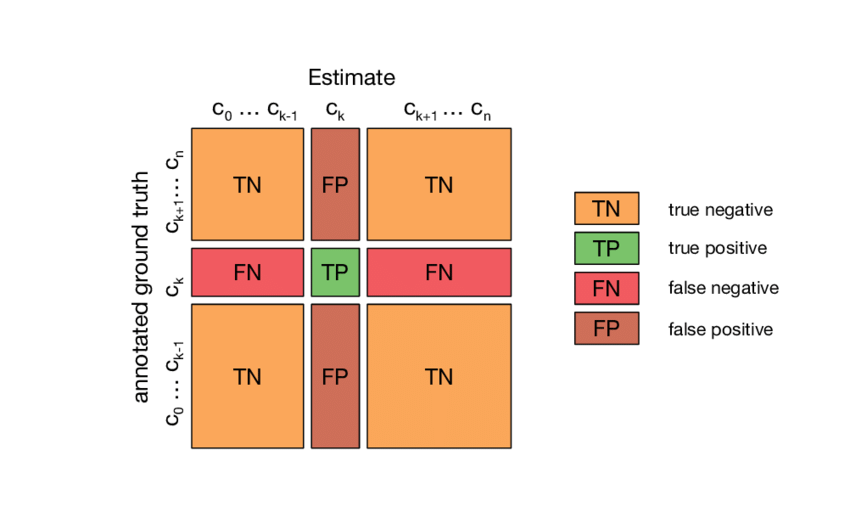
\includegraphics[width=1\linewidth]{images/Confusion_matrix_explanation.png}
		\caption{Multiclass confusion matrix, source: \small \textit{Activity, Context, and Plan Recognition with Computational Causal Behaviour Models - Scientific Figure on ResearchGate}}
    \end{figure}
    
    % What can we see from the confusion matrix?
    % which faces are being mixed up (if any)?
    % why that might be?
     

\end{document}